\section{Chiamate di Sistema}
Le chiamate di sistema forniscono un'interfaccia tra i programmi e i servizi offerti dal sistema operativo.

Questo permette al programmatore di chiamare le funzioni da linguaggi di programmazione ad alto livello (C o C++) anche se l'implementazione può essere stata fatta ad esempio in assembly.

\subsection{Implementazione}
Dal punto di vista implementativo viene assegnato un numero ad ogni \textit{system call} e il sistema operativo tiene una tabella che associa numeri al codice che gestisce la chiamata a sistema.

\begin{figure}[H]
    \centering
    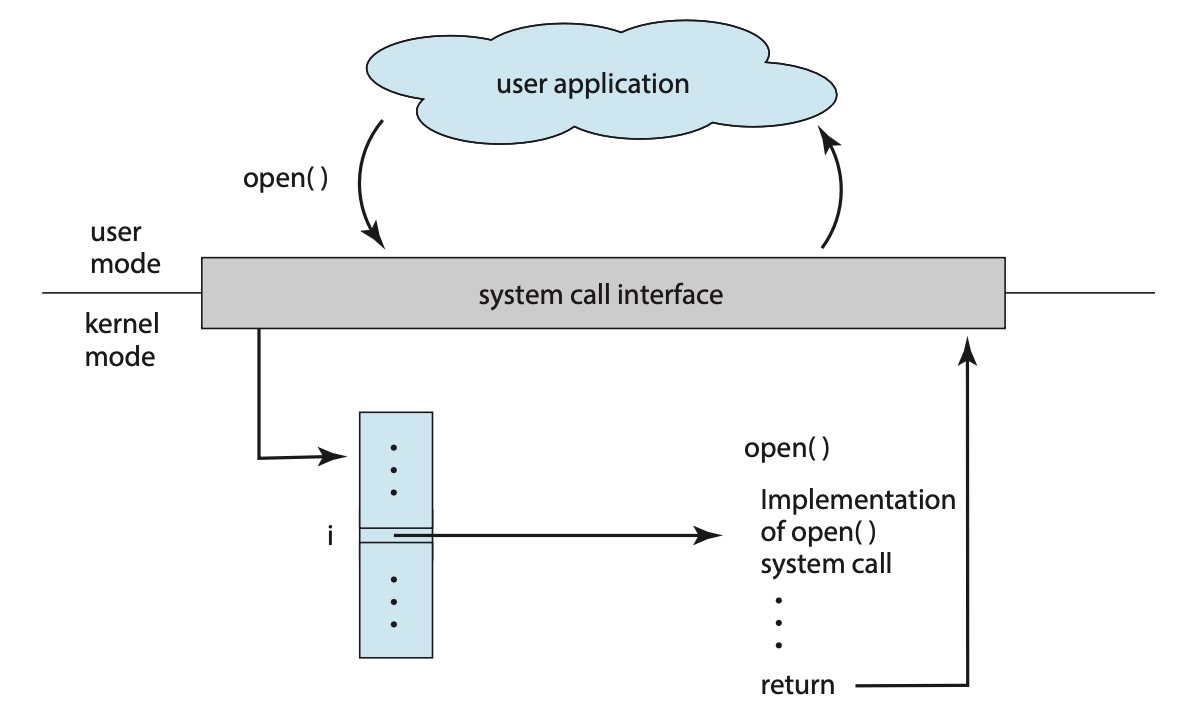
\includegraphics[width=0.65\linewidth]{assets/systemcall.jpg}
    \caption{La gestione della chiamata a sistema \texttt{open()}}
\end{figure}

Spesso è necessario fornire più informazioni della semplice chiamata. Il tipo e la quantità di dati che devono essere forniti alla \textit{system call} possono variare molto.

\spacer
Ci sono diverse soluzioni a questo problema:
\begin{sitemize}
    \item \textbf{Utilizzare i registri}, per quanto sia il metodo più semplice, limita numero e dimensione dei parametri.
    \item Memorizzazione dei parametri su un \textbf{blocco di memoria} e passaggio dell'indirizzo del blocco utilizzando un registro (Linux e Solaris).
    \item \texttt{Push} dei parametri nello \textbf{stack} da parte del programma e poi \textit{}t{pop} da parte del sistema operativo.
\end{sitemize}

\subsection{Application Programming Interface}
Gli sviluppatori spesso non vedono l'implementazione di queste funzioni, che spesso risultano essere estremamente complesse anche per azioni relativamente semplici.

I programmi e i loro sviluppatori interagiscono con delle \textit{Application Programming Interface (API)}, un set di funzioni che sono disponibili al programmatore.

\spacer
L'utilizzo di un'API permette all'utente di non preoccuparsi dei dettagli implementativi e permette una maggiore portabilità del programma ad altri sistemi operativi.

\begin{note}
    Alcune delle API più diffuse ed utilizzate sono la \textit{Win64 API} per Windows, \textit{POSIX API} per Unix, Linux e MacOS e la \textit{Java API} per la \textit{Java Virtual Machine}.
\end{note}

\subsection{Tipologie di Chiamate a Sistema}

Le chiamate a sistema possono essere approssimativamente raggruppate in 6 categorie principali:
\begin{sitemize}
    \item \textbf{Controllo dei Processi:}

    Permette di creare, caricare, eseguire, far attendere e terminare un processo. Inoltre permette di leggere e modificare gli attributi del processo (priorità, tempo di esecuzione, $\ldots$), assegnare/rilasciare memoria e inviare segnali.

    \item \textbf{Gestione delle informazioni:}

    Permette di ottenere informazioni di sistema, la lettura/modifica dell'ora e della data, la lettura/modifica degli attributi di processi, file e dispositivi.

    \item \textbf{Comunicazione:}

    Permette l'apertura/chiusura di una connessione, l'invio/ricezione di messaggi, inserimento/esclusione di dispositivi remoti, condivide informazioni sullo stato dei trasferimenti e gestisce la condivisione della memoria.

    \item \textbf{Gestione dei file:}

    Permette la creazione/eliminazione/apertura/chiusura/lettura/scrittura di file e condivide gli attributi dei file.

    \item \textbf{Gestione dei dispositivi I/O:}

    Permette la richiesta e rilascio di un dispositivo, la lettura e scrittura dei dati e condivide gli attributi di un dispositivo.
\end{sitemize}
